\newpage
\section{Lossless Impedance Functions}
\subsection{Hamiltonians Derived from Lossless Reciprocal Impedance Functions}\label{section:impedance_hamiltonian}

We will primarily be studying the partial fraction expansion of a general lossless impedance function and its synthesis that is presented in \cite[Chapter 7]{newcomb}. In the Laplace domain with $s=\sigma+i\omega$, the partial fraction expansion of a multiport lossless impedance function is given by
\begin{equation}\label{eq:general_impedance}
    \vb{Z}(s) = \frac{\vb{A}_0}{s} + s\vb{A}_\infty + \vb{B}_\infty + \sum_{k=1}^{M} \frac{s\vb{A}_k + \vb{B}_k}{s^2 + \omega_{R_k}^2}
\end{equation}
where the $\vb{A}$ matrices are real, positive semidefinite, and symmetric, and the $\vb{B}$ matrices are real and antisymmetric. The resonant modes of the network have frequency $\omega_{R_k}$. In our modeling of superconducting circuits, we will make the following assumptions that will put some restrictions on (\ref{eq:general_impedance}) which reduce it to a simpler form:
\begin{enumerate}
    \item Our models will have a reciprocal response such that all matrices $\vb{B}_i = 0$. It is clear that in this case, $\vb{Z}(s)^T=\vb{Z}(s)$.
    \item Each port of our network will have a non-zero shunt capacitance. This is physically motivated and the same assumption is made in \cite{solgun_sirf,sherbrooke_sirf}. The result is that the DC residue $\vb{A}_0$ is of full-rank and positive definite.
    \item The poles of the network at infinite frequency can be reasonably well approximated by finite frequency poles that are outside of the relevant frequency range of our devices. Thus, the residue $\vb{A}_\infty$ can be treated as a finite frequency pole. Inclusion of the infinite frequency residue will lead to a circuit Lagrangian with a singular capacitance matrix for which we cannot write a Hamiltonian (see Appendix \ref{appendix:infty_freq_residue}).
    \item A residue $\vb{A}_k$ corresponding to resonant mode $k$ is restricted to being rank-1. If degenerate resonant modes are present, multiple rank-1 residues can be associated with a single resonant frequency. Generally, parasitic or nonsymmetric coupling in physical models will break these degeneracies (see Appendix \ref{appendix:degen_res_mode}).
\end{enumerate}
The assumptions listed are based on the physical models of the devices that we will consider as explained in the previous section. With the above assumptions in mind, we now have the following lossless reciprocal impedance function:
\begin{equation}\label{eq:impedance}
    \vb{Z}(s) = \frac{\vb{R}_0}{s} + \sum_{k=1}^M \frac{s \vb{R}_k}{s^2 + \omega_{R_k}^2}
\end{equation}
An $N$-port impedance function (\ref{eq:impedance}) can be synthesized using a multiport canonical Cauer circuit as shown in Fig.\ \ref{fig:cauer_circuit} in the same way as \cite{solgun_sirf}. The following relationships link the residues and resonant frequencies of the impedance function (\ref{eq:impedance}) to the lumped elements of the synthesized circuit in Fig.\ \ref{fig:cauer_circuit}:
\begin{align}
    \vb{C}_0 &= \diag(C_1, \dots, C_N) \\
    \vb{R}_0 &=  \vb{U} \vb{C}_0^{-1} \vb{U}^T \label{eq:DC_residue}\\
    \vb{r}_k &= (r_{k1}, \dots, r_{kN}) \label{eq:row_R}\\
    \vb{R}_k &= \vb{r}_k^T \vb{r}_k \\
    L_{R_k} &= 1/\omega_{R_k}^2 \\
    C_{R_k} &= 1 \label{eq:C_R}
\end{align}

\definecolor{nodecolor}{HTML}{990000}
\definecolor{junctioncolor}{HTML}{224466}
\begin{figure}[!p]
    \centering
    \begin{circuitikz}[line width=1pt]
    \ctikzset{american}
    \ctikzset{bipoles/thickness=1, bipoles/length=1cm}
    \ctikzset { label/align = straight }

    % ------------------------------- Port 1 Branch ------------------------------ %
    {\color{junctioncolor} 
    % \draw (0,-1) -- (0,1);
    \draw (0,-1) to[generic, color=junctioncolor] (0,1);
    \node[anchor=west] at (0.15,0) {\Large $U_1$}; 
    }
    \draw (2,7.5) to[L, name=TJC1] (2,6.5) -- (2,2.5) to[L, name=r11] (2,1.5) -- (2,0.5);
    \draw (2,-0.5) -- (2,-1.5) to[L, name=rm1] (2,-2.5) -- (2,-4.5) to[L, name=t11] (2,-5.5) -- (2,-5.75);
    \draw (2,-6.25) -- (2,-6.5) to[L, name=tn1] (2,-7.5);
    \draw[rounded corners=.5cm] (2,7.4) -- (2,8) -- (0,8) to[short, -o] (0,1);
    \draw[rounded corners=.5cm] (2,-7.4) -- (2,-8) -- (0,-8) to[short, -o] (0,-1);
    
    \node[circle, fill=nodecolor, inner sep=0pt,minimum size=5pt, label={[label distance=-0.1cm]above:{\Large \color{nodecolor} $\Phi_{P_1}$}}] at (1,8) {};
    
    \node[anchor=east] at (2,7) {\Large\color{nodecolor} $\Phi_{PC_1}\bigg($};
    
    \draw[thick, double] (TJC1.core east) -- (TJC1.core west);
    \draw[thick, double] (r11.core east) -- (r11.core west);
    \draw[thick, double] (rm1.core east) -- (rm1.core west);
    \draw[thick, double] (t11.core east) -- (t11.core west);
    \draw[thick, double] (tn1.core east) -- (tn1.core west);
    
    % \node at (3,6) {$\ddots$};
    \node at (2,.1) {$\vdots$};
    \node at (2,-5.9) {$\vdots$};
    \node at (3,0) {\dots};
    \node[anchor=west] at (1.97,7.65) {1};
    \node[anchor=west] at (1.97,2.65) {$r_{11}$};
    \node[anchor=west] at (1.97,-1.35) {$r_{M1}$};
    \node[anchor=west] at (1.97,-4.35) {$t_{11}$};
    \node[anchor=west] at (1.97,-6.35) {$t_{N1}$};

    % ------------------------------- Port N Branch ------------------------------ %
    {\color{junctioncolor}
    % \draw (4,-1) -- (4,1);
    \draw (4,-1) to[generic, color=junctioncolor] (4,1);
    \node[anchor=west] at (4.15,0) {\Large $U_N$};}
    \draw (6,5.5) to[L, name=TJCN] (6,4.5) -- (6,2.5) to[L, name=r1n] (6,1.5) -- (6,0.5);
    \draw (6,-0.5) -- (6,-1.5) to[L, name=rmn] (6,-2.5) -- (6,-4.5) to[L, name=t1n] (6,-5.5) -- (6, -5.75);
    \draw (6, -6.25) -- (6,-6.5) to[L, name=tnn] (6,-7.5);
    \draw[rounded corners=.5cm] (6,5.4) -- (6,8) -- (4,8) to[short, -o] (4,1);
    \draw[rounded corners=.5cm] (6,-7.4) -- (6,-8) -- (4,-8) to[short, -o] (4,-1);
    
    \node[circle, fill=nodecolor, inner sep=0pt,minimum size=5pt, label={[label distance=-0.1cm]above:{\Large \color{nodecolor} $\Phi_{P_N}$}}] at (5,8) {};
    
    \node[anchor=east] at (6,5) {\Large\color{nodecolor} $\Phi_{PC_N}\bigg($};

    \draw[thick, double] (TJCN.core east) -- (TJCN.core west);
    \draw[thick, double] (r1n.core east) -- (r1n.core west);
    \draw[thick, double] (rmn.core east) -- (rmn.core west);
    \draw[thick, double] (t1n.core east) -- (t1n.core west);
    \draw[thick, double] (tnn.core east) -- (tnn.core west);

    \node at (6,.1) {$\vdots$};
    \node at (6,-5.9) {$\vdots$};
    \node[anchor=west] at (5.97,5.65) {1};
    \node[anchor=west] at (5.97,2.65) {$r_{1N}$};
    \node[anchor=west] at (5.97,-1.35) {$r_{MN}$};
    \node[anchor=west] at (5.97,-4.35) {$t_{1N}$};
    \node[anchor=west] at (5.97,-6.35) {$t_{NN}$};

    % -------------------------------- Cap Stage 1 ------------------------------- %
    \draw (8,6.25) -- (8,6.5) to[L, name=u11] (8, 7.5);
    \draw (8,5.75) -- (8,5.5) to[L, name=un1, mirror] (8,4.5);
    \draw[rounded corners=.5cm] (8, 7.4) -- (8,8) -- (9.5,8) to[C={\Large $C_1$}, name=c1] (9.5,4) -- (8,4) -- (8,4.6);
    \node[circle, fill=nodecolor, inner sep=0pt,minimum size=5pt, label={[label distance=-0.1cm]above:{\Large \color{nodecolor} $\Phi_{C_1}$}}] at (8.75,8) {};
    \node[anchor=east] at (8,7.65) {\small $U_{11}$};
    \node[anchor=east] at (8,5.65) {\small $U_{N1}$};
    \draw[thick, double] (u11.core east) -- (u11.core west);
    \draw[thick, double] (un1.core east) -- (un1.core west);
    \node at (8,6.1) {\vdots};

    \node at (11.05,6) {\dots};

    % -------------------------------- Cap Stage N ------------------------------- %
    \draw (12.5,6.25) -- (12.5,6.5) to[L, name=u11] (12.5, 7.5);
    \draw (12.5,5.75) -- (12.5,5.5) to[L, name=un1, mirror] (12.5,4.5);
    \draw[rounded corners=.5cm] (12.5, 7.4) -- (12.5,8) -- (14,8) to[C={\Large $C_N$}, name=c1] (14,4) -- (12.5,4) -- (12.5,4.6);
    \node[circle, fill=nodecolor, inner sep=0pt,minimum size=5pt, label={[label distance=-0.1cm]above:{\Large \color{nodecolor} $\Phi_{C_N}$}}] at (13.25,8) {};
    \node[anchor=east] at (12.5,7.65) {\small $U_{1N}$};
    \node[anchor=east] at (12.5,5.65) {\small $U_{NN}$};
    \draw[thick, double] (u11.core east) -- (u11.core west);
    \draw[thick, double] (un1.core east) -- (un1.core west);
    \node at (12.5,6.1) {\vdots};

    % ----------------------------- Resonant Stage 1 ----------------------------- %
    \draw (8,1.5) to[L, name=res1] (8,2.5);
    {
    \ctikzset{cute}
    \draw[rounded corners=.5cm] (8,2.4) -- (8,3) -- (11,3) -- (12,3) to[L={\Large $L_{R_1}$}] (12,1) -- (8,1) -- (8,1.6);
    }
    \draw (10,3) to[C={\Large $C_{R_1}$}] (10,1);
    \node[circle, fill=nodecolor, inner sep=0pt,minimum size=5pt, label={[label distance=-0.1cm]above:{\Large \color{nodecolor} $\Phi_{R_1}$}}] at (10,3) {};

    \draw[thick, double] (res1.core west) -- (res1.core east);
    \node[anchor=east] at (8.0125,2.65) {1};
    
    % ----------------------------- Resonant Stage N ----------------------------- %
    \draw (8,-2.5) to[L, name=resN] (8,-1.5);
    {
    \ctikzset{cute}
    \draw[rounded corners=.5cm] (8,-1.6) -- (8,-1) -- (12,-1) to[L={\Large $L_{R_N}$}] (12,-3) -- (11,-3) -- (8,-3) -- (8,-2.4);
    }
    \draw (10,-1) to[C={\Large $C_{R_N}$}] (10,-3);
    \node[circle, fill=nodecolor, inner sep=0pt,minimum size=5pt, label={[label distance=-0.1cm]above:{\Large \color{nodecolor} $\Phi_{R_N}$}}] at (10,-1) {};

    \draw[thick, double] (resN.core west) -- (resN.core east);
    \node[anchor=east] at (8.0125,-1.35) {1};
    \node at (10,.1) {$\vdots$}; % or should the vertical spacing be .3?

    % ----------------------------- Inductive Stage 1 ---------------------------- %
    \draw (8, -5.5) to[L, name=L1] (8, -4.5);
    {
    \ctikzset{cute}
    \draw[rounded corners=.5cm] (8,-5.4) -- (8,-8) -- (9.5,-8) to[L,l_={\Large $L_1$}, mirror] (9.5,-4) -- (8,-4) -- (8,-4.6);
    }
    \draw[thick, double] (L1.core east) -- (L1.core west);
    \node[circle, fill=nodecolor, inner sep=0pt,minimum size=5pt, label={[label distance=-0.1cm]above:{\Large \color{nodecolor} $\Phi_{L_1}$}}] at (8.75,-4) {};
    \node[anchor=east] at (8.0125,-4.35) {1};
    \node at (11.15,-6) {\dots};

    % % ----------------------------- Inductive Stage N ---------------------------- %
    \draw (12.5, -7.5) to[L, name=LN] (12.5, -6.5);
    {
    \ctikzset{cute}
    \draw[rounded corners=.5cm] (12.5,-7.4) -- (12.5,-8) -- (14,-8) to[L,l_={\Large $L_N$}, mirror] (14,-4) -- (12.5,-4) -- (12.5,-6.6);
    }
    \draw[thick, double] (LN.core east) -- (LN.core west);
    \node[circle, fill=nodecolor, inner sep=0pt,minimum size=5pt, label={[label distance=-0.1cm]above:{\Large \color{nodecolor} $\Phi_{L_N}$}}] at (13.25,-4) {};
    \node[anchor=east] at (12.5125,-6.35) {1};
\end{circuitikz}
\caption{The canonical Cauer circuit that represents the synthesis of the impedance function (\ref{eq:impedance}) with the ports shunted by potentials that are functions of the port fluxes: $U_i(\Phi_{J_i})$. The multiport transformer with turns ratios in matrix $\vb{U}$ couple the ports of the network to the purely capacitive stage that is related to the DC residue $\vb{R}_0$. The turns ratio matrix $\vb{R}$ represents the multiport transformer that couples the ports to the resonant modes. The residue at infinite frequency corresponds to the purely inductive stage which is included here to help motivate why it can be neglected. In practice, parasitic capacitances will bring the infinite frequency pole to finite frequency and thus this purely inductive stage can be included in the resonant stage. In Appendix \ref{appendix:infty_freq_residue}, we can also see that if one attempts to construct a Hamiltonian when the purely inductive stage is present, the resulting capacitance matrix is singular.}
\label{fig:cauer_circuit}
\end{figure}

$\vb{U}$ and $\vb{R}$ correspond to the turns ratios of the multiport Belevitch transformers that correspond to the purely capacitive and resonant stages, respectively, as shown in Fig.\ \ref{fig:cauer_circuit}. Furthermore, $\vb{r}_k$ in (\ref{eq:row_R}) is defined as row $k$ of the turns ratio matrix $\vb{R}$. This definition of the residues $\vb{R}_k$ guarantees that they are rank-1.

Our goal is to make a quantum mechanical model of the lumped element circuit that corresponds to the impedance function. Before doing this, it is first worth discussing how this is generally done for lumped element circuits in the context of circuit-QED \cite{vool_devoret,cqed_lecture_notes}. 

\begin{figure}[!h]
    \centering
    \begin{subfigure}{.4\textwidth}
        \centering
        \begin{circuitikz}[line width=1.5pt]
            \ctikzset{american}
            \ctikzset{bipoles/thickness=1, bipoles/length=2cm}
            \ctikzset { label/align = straight }

            \draw[color=white] (0,4) to (0,-0.25);

            \draw (0,3) to[generic] (0,0);

            \node[circle, fill=nodecolor, inner sep=0pt,minimum size=5pt] at (0,3) {};
            \node[circle, fill=nodecolor, inner sep=0pt,minimum size=5pt] at (0,0) {};

            \node[color=nodecolor] at (-1,3) {\LARGE $\boldsymbol{+}$};
            \node[color=nodecolor] at (-1,0) {\LARGE $\boldsymbol{-}$};
            \node[color=nodecolor] at (-1,1.5) {\Large $v_{b}$};
            
            \draw [color=nodecolor] [-stealth] (0.6,2.25) to (0.6,0.75);
            \node[color=nodecolor] at (1,1.5) {\Large $i_{b}$};

            \node[color=nodecolor] at (0,1.5) {$b$};

        \end{circuitikz}
        \caption{}
        \label{fig:branch_element}
    \end{subfigure}%
    \begin{subfigure}{.4\textwidth}
        \centering
        \begin{circuitikz}[line width=1.5pt]
            \ctikzset{american}
            \ctikzset{bipoles/thickness=1, bipoles/length=2cm}
            % \ctikzset{bipoles/inductors/core distance=4pt}
            \ctikzset { label/align = straight }
            \draw[color=white] (0,-1.75) to (0,2.5);
            \draw (0,0) node[transformer core] (T) {};
            \node[circle, fill=nodecolor, inner sep=0pt,minimum size=5pt, label={[label distance=0cm]above:{\Large \color{nodecolor} $i_{b_1}$}}] at (-1.5,1.5) {};
            \draw[color=nodecolor] [-stealth](-1.15,2) to (-.75,2);
            \node[circle, fill=nodecolor, inner sep=0pt,minimum size=5pt] at (-1.5,-1.5) {};
            \node[circle, fill=nodecolor, inner sep=0pt,minimum size=5pt, label={[label distance=0cm]above:{\Large \color{nodecolor} $i_{b_2}$}}] at (1.5,1.5) {};
            \node[circle, fill=nodecolor, inner sep=0pt,minimum size=5pt] at (1.5,-1.5) {};
            \draw[color=nodecolor] [-stealth](1.15,2) to (.75,2);
            
            \node[color=nodecolor] at (-1.5,1) {\LARGE $\boldsymbol{+}$};
            \node[color=nodecolor] at (-1.5,-1) {\LARGE $\boldsymbol{-}$};
            \node[color=nodecolor] at (-1.5,0) {\Large $v_{b_1}$};    

            \node[color=nodecolor] at (1.5,1) {\LARGE $\boldsymbol{+}$};
            \node[color=nodecolor] at (1.5,-1) {\LARGE $\boldsymbol{-}$};
            \node[color=nodecolor] at (1.5,0) {\Large $v_{b_2}$};

            \node at (0,1.1) {\scriptsize $N_1:N_2$};

        \end{circuitikz}
        \caption{}
        \label{fig:ideal_transformer}
    \end{subfigure}
    \caption{(a) General lumped-element branch $b$. (b) Two-branch ideal transformer element with turns ratio $t=N_2/N_1$.}
    \label{fig:branch_and_transformer}
\end{figure}

Consider a general lumped element as pictured in Fig.\ \ref{fig:branch_element} with the voltage across the branch $v_b(t)$. This is defined as the differences between the node voltages at the top and bottom of the pictured branch. To make a quantum mechanical model of a circuit with branch elements as shown, we would like to obtain a Hamiltonian that we can quantize. To do this, we will first generally find a Lagrangian for our circuit to which we apply a Legendre transformation. The degrees of freedom for this Lagrangian are flux variables that are defined in terms of branch or node voltages:
\begin{equation}
    \Phi_b(t) = \int_{-\infty}^t v_b(t')\; dt'
\end{equation}
We assume that the electromagnetic fields are not present for $t \rightarrow -\infty$. Using the flux variables corresponding to branches of a lumped element circuit, we can write a Lagrangian $\mathcal{L} = T - U$ that contains kinetic and potential energy terms for various elements. Throughout this thesis we will primarily be concerned with three two-terminal elements: capacitors, inductors, and Josephson junctions. The capacitor and inductor are linear elements, while the Josephson junction is nonlinear. The kinetic and potential energies of branches with a capacitor $C$, inductor $L$ and Josephson junction are defined in terms of branch fluxes as:
\begin{align}
    T_C(t) &= \frac{1}{2}C\dot{\Phi}_b^2(t) \\
    U_L(t) &= \frac{1}{2L}\Phi_b^2(t) \\ 
    U_J(t) &= -E_J \cos(\frac{2\pi}{\Phi_0} \Phi_b)
\end{align}
where $\Phi_0=h/2e$ is the superconducting flux quantum, and $E_J=\Phi_0 I_c/2\pi$ is the Josephson junction energy defined in terms of its critical current. In our lumped element circuits, we will also consider ideal transformers as shown in Fig.\ \ref{fig:ideal_transformer}. This element constrains the two branch voltages across its terminals such that $v_{b_2} = tv_{b_1}$ where $t=N_2/N_1 \in \mathbb{R}$ is the turns ratio of the ideal transformer. This places a similar constraint on the branch fluxes: $\Phi_{b_2} = t\Phi_{b_1}$.

Using the above potential and kinetic energies for capacitors and inductors, as well as the relationship between two branches coupled with an ideal transformer, we can find a circuit Hamiltonian that will later on allow us to characterize the behavior of qubit networks. We will arrive at the same Hamiltonian presented in \cite{solgun_sirf} where a different method was used to treat the multiport transformers \cite{burkard_circuit_2005,multiport_impedance_quantization}. To start, we write the Lagrangian for the synthesized circuit of in Fig.\ \ref{fig:cauer_circuit} using the node fluxes of the purely capacitive stage $\Phi_{C_i}$, the resonant stage $\Phi_{R_i}$, and the elements shunting the ports $\Phi_{P_i}$:
\begin{equation}\label{eq:impedance_lagrangian}
    \mathcal{L} = \frac{1}{2}\dot{\vb{\Phi}}_C^T \vb{C}_0 \dot{\vb{\Phi}}_C^{\phantom{^T}} + \frac{1}{2}\dot{\vb{\Phi}}_R^T \vb{C}_R \dot{\vb{\Phi}}_R^{\phantom{^T}} - \frac{1}{2}\vb{\Phi}_R^T \vb{M}_R \vb{\Phi}_R^{\phantom{^T}} - \sum_{i=1}^N U_i(\Phi_{P_i})
\end{equation}
where $\vb{C}_R = \diag(C_{R_1}, \dots, C_{R_M})$, $\vb{M}_R = \diag(L_{R_1}^{-1}, \dots, L_{R_M}^{-1})$, and the elements of the $\vb{\Phi}$ vectors contain the node fluxes of capacitive and resonant stages in the Cauer circuit. The potential functions $U_i(\Phi_{P_i})$ correspond to lumped elements that shunt the ports of the impedance with some arbitrary potential. This arbitrary potential can correspond to both linear or nonlinear elements. The next step is to make a substitution that returns a Lagrangian dependent only on the port fluxes $\Phi_{P_i}$ and the resonant stage fluxes $\Phi_{R_i}$. The substitution that we make invokes the constraint that an ideal transformer puts on the two branches that it couples. For example, the constraint between the flux variable of the branch $\Phi_{C_1}$ and the ideal transformer branches at the ports gives:
\begin{equation}
    \Phi_{C_1} = U_{11}\Phi_{PC_1} + \dots + U_{N1}\Phi_{PC_N}
\end{equation}
Using this reasoning for the rest of the branches coupled using ideal transformers, we find the following constraints for the branch and node flux vectors:
\begin{align}
    \vb{\Phi}_C &= \vb{U}^T \vb{\Phi}_{PC} \\
    \vb{\Phi}_{PC} &= \vb{\Phi}_P - \vb{R}^T \vb{\Phi}_R
\end{align}
This allows for the substitution $\vb{\Phi}_C \rightarrow \vb{U}^T (\vb{\Phi}_P - \vb{R}^T\vb{\Phi}_R)$, so we can eliminate $\vb{\Phi}_C$ from the first term in (\ref{eq:impedance_lagrangian}):
\begin{equation}
    \dot{\vb{\Phi}}_C^T \vb{C}_0 \dot{\vb{\Phi}}_C^{\phantom{^T}} = \dot{\vb{\Phi}}_P^T \vb{R}_0^{-1} \dot{\vb{\Phi}}_P^{\phantom{^T}} - \dot{\vb{\Phi}}_P^{T} \vb{R}_0^{-1} \vb{R}^T \dot{\vb{\Phi}}_R^{\phantom{^T}} - \dot{\vb{\Phi}}_R^{T} \vb{R}^T \vb{R}_0^{-1} \dot{\vb{\Phi}}_P^{\phantom{T}} + \dot{\vb{\Phi}}_R^{T} \vb{R} \vb{R}_0^{-1} \vb{R}^T \dot{\vb{\Phi}}_R^{\phantom{^T}}
\end{equation}
Above we have also eliminated $\vb{C}_0$ using (\ref{eq:DC_residue}). Applying a Legendre transformation to the resulting Lagrangian will yield the following circuit Hamiltonian in agreement with \cite{solgun_sirf}:
\begin{equation}\label{eq:impedance_hamiltonian}
    \mathcal{H} = \frac{1}{2} \vb{Q}^T \vb{C}^{-1} \vb{Q} + \frac{1}{2} \vb{\Phi}^T \vb{M} \vb{\Phi} + \sum_{i=1}^N U_i(\Phi_{P_i})
\end{equation}
where we have now defined the conjugate variables $Q_{P_i} = \partial \mathcal{L}/\partial \Phi_{P_i}$ and the following vectors and matrices:
\begin{align}
    \vb{\Phi} &= (\Phi_{P_1}, \dots, \Phi_{P_N}, \Phi_{R_1}, \dots, \Phi_{R_M})^T \\
    \vb{Q} &= (Q_{P_1}, \dots, Q_{P_N}, Q_{R_1}, \dots, Q_{R_M})^T \\
    \vb{C} &= \mqty( \vb{R}_0^{-1} & -\vb{R}_0^{-1}\vb{R}^T \\ -\vb{R} \vb{R}_0^{-1} & \vb{C}_R + \vb{R}\vb{R}_0^{-1}\vb{R}^T) \label{eq:impedance_cap}\\
    \vb{M} &= \mqty(\vb{0}_{N\times N} & \vb{0}_{N\times M} \\ \vb{0}_{M\times N} & \vb{M}_R)
\end{align}
We expect that a capacitance matrix should always be positive definite \cite{pos_cap}. For our choice of $\vb{C_R} = \mathds{1}_{M\times M}$ in (\ref{eq:C_R}), $\vb{C}$ will always be positive definite ($\vb{C} > 0$). This is the case since $\vb{R}_0 > 0$ and the Schur complement $\vb{C}/\vb{R}_0^{-1}=\mathds{1}_{M\times M} > 0$ \cite[Theorem 1.12]{schur_comp}. Also, since $\vb{C} > 0$, it is invertible, which allows us to write the final Hamiltonian (\ref{eq:impedance_hamiltonian}). Computing the inverse of $\vb{C}$, we find \cite[Proposition 2.8.7]{matrix_mathematics}:
\begin{equation}\label{eq:impedance_cap_inverse}
    \vb{C}^{-1} = \mqty( 
        \vb{R}_0 + \vb{R}^T \vb{C}_R^{-1} \vb{R} & \vb{R}^T \vb{C}_R^{-1} \\ 
        \vb{C}_R^{-1} \vb{R} & \vb{C}_R^{-1}
    ) = 
    \mqty( 
        \vb{R}_0 + \vb{R}^T \vb{R} & \vb{R}^T  \\ 
         \vb{R} & \mathds{1}_{M\times M}
    )
\end{equation}


\newpage
\subsection{Cascade Synthesis of the Lossless Reciprocal Impedance Function}\label{section:cascade_synthesis}
One interesting aspect of the Hamiltonian (\ref{eq:impedance_hamiltonian}) derived in the previous section is that it defines an alternative synthesis of the impedance function (\ref{eq:impedance}). Before diving into the details of the synthesis itself, we first need to discuss and define the Maxwell and mutual capacitance matrices. Given a network of $N$ nodes that each have a capacitance to ground $C_{g,i}$ and node coupling capacitances $C_{ij}$, the Maxwell capacitance matrix $\vb{C}$ gives the relationship between the voltages and charges at the nodes \cite{pos_cap, ruehli_cap}
\begin{equation}
    \vb{Q} = \vb{C} \vb{V}
\end{equation}
The matrix elements of the Maxwell capacitance matrix are defined in the following way:
\begin{equation}
    (\vb{C})_{ij} = \begin{cases}
    C_{g,i} + \sum_{k \neq i} C_{ik} & i = j\\
    -C_{ij} & i \neq j
    \end{cases}
\end{equation}
We can also define the mutual capacitance matrix $\vb{C}_{mut}$ with matrix elements
\begin{equation}
    (\vb{C}_{mut})_{ij} = \begin{cases}
        C_{g,i} & i=j\\
        C_{ij} & i \neq j
    \end{cases}
\end{equation}
In electromagnetic or circuit modeling software, this mutual capacitance matrix is sometimes called the SPICE capacitance matrix. It simply gives the mutual capacitance between the nodes of the network. It is easy to convert between the two types of matrices and the conversion is also reciprocal:
\begin{equation}
    (\vb{C}_{mut})_{ij} = \begin{cases}
        \sum_{k=0}^N(\vb{C})_{ik} & i=j \\
        -(\vb{C})_{ij} & i \neq j
    \end{cases}
\end{equation}
Now that the Maxwell and mutual capacitance matrices are defined, we can discuss the alternative synthesis of the impedance function (\ref{eq:impedance}). Disregarding the potential contribution to the Hamiltonian (\ref{eq:impedance_hamiltonian}) from the elements shunting the ports, we can see that the Hamiltonian describes a cascade network as shown in Fig.\ \ref{fig:cascade_impedance}. The first network in the cascade is a purely capacitive $(N+M)$ port network that has a Maxwell capacitance matrix $\vb{C}$ defined by (\ref{eq:impedance_cap}). A synthesis of this portion of the cascade can be easily found by converting the Maxwell form capacitance matrix to its mutual form. This purely capacitive network is then shunted by inductances $L_{R_k}=1/\omega_{R_k}^2$. We will refer to this network structure as a CL cascade.

\begin{figure}[h!]
    \centering
    \begin{circuitikz}[line width=1pt]
        \ctikzset{bipoles/thickness=1, bipoles/length=1cm}
        \ctikzset { label/align = straight }
        
        % ---------------------------- Capacitive Network ---------------------------- %
        \draw[rounded corners=.5cm] (0,2) -- (0,4.5) -- (7,4.5) -- (7,0) -- (0,0) -- (0,2);
        \node at (3.5,2.25) {$\vb{C} = \mqty( \vb{R}_0^{-1} & -\vb{R}_0^{-1}\vb{R}^T \\ -\vb{R} \vb{R}_0^{-1} & \mathds{1}_{M\times M} + \vb{R}\vb{R}_0^{-1}\vb{R}^T)$};

        % --------------------------- Inductive Network Box -------------------------- %
        \draw[rounded corners=0.5cm] (9,2) -- (9,4.5) -- (11,4.5) -- (11,0) -- (9,0) -- (9,2);
        \draw (9,3) -- (9.6,3) to[L,l_=$\dfrac{1}{\omega_{R_1}^2}$, mirror, label distance=0.25cm] (9.6,4) -- (9,4);
        \draw (9,0.5) -- (9.6,0.5) to[L,l_=$\dfrac{1}{\omega_{R_M}^2}$, mirror, label distance=0.25cm] (9.6,1.5) -- (9,1.5);

        % ------------------------------ Left Lower Port ----------------------------- %
        \draw (0,0.5) to[short, -o] (-1,0.5);
        \draw (0,1.5) to[short, -o] (-1,1.5);

        % ------------------------------ Left Upper Port ----------------------------- %
        \draw (0,3) to[short, -o] (-1,3);
        \draw (0,4) to[short, -o] (-1,4);

        % ----------------------------- Middle Lower Port ---------------------------- %
        \draw (7,0.5) to[short, -o] (8,0.5) -- (9,0.5);
        \draw (7,1.5) to[short, -o] (8,1.5) -- (9,1.5);

        % ----------------------------- Middle Upper Port ---------------------------- %
        \draw (7,3) to[short, -o] (8,3) -- (9,3);
        \draw (7,4) to[short, -o] (8,4) -- (9,4);

        \node at (-0.5,2.35) {$\vdots$};
        \node at (8,2.35) {$\vdots$};
        \node at (10,2.35) {$\vdots$};

        \draw[decoration={brace}, decorate] (-1.25,0.25) -- (-1.25,4.25);
        \node[rotate=90] at (-1.75, 2.25) {$N$ ports};

    \end{circuitikz}
    \caption{Cascade synthesis for the impedance function (\ref{eq:impedance}). }
    \label{fig:cascade_impedance}
\end{figure}
What is interesting about the cascade synthesis presented above is that it removes the multiport transformers present in the Cauer synthesis of the impedance function. However, the caveat of this transformerless synthesis is that it is possible to end up with \textit{negative} values for the capacitances in the mutual capacitance matrix and thus negative capacitors in the cascade synthesis. Including negative inductive, capacitive or resistive circuit elements in the synthesis of a network is not a new idea. For example, in the Brune method of synthesis, negative inductances or capacitances may appear. However, these elements can be absorbed into the rest of the network to form mutual inductances or ideal transformers such that the final synthesis contains only passive elements \cite{brune_synthesis}, \cite[Chapter 9.4]{guillemin_synthesis}. This requirement that the final representation of a network should contain only passive circuit elements has shaped much of the history of network synthesis and is in general the agreed upon approach \cite[Chapter 1.2]{cauer_linear_comm}. However, for our use case and synthesized cascade network, even though there may be negative capacitances present, we have seen that the Maxwell capacitance matrix of the network is positive definite, and therefore the \textit{overall} network is passive which is what matters in our case. Having negative capacitances is a consequence of the fact that the turns ratios present in the multiport transformers can take positive and negative values. We can motivate this idea further using two simple examples.

First, we consider the following two-port impedance function:
\begin{equation}\label{eq:impedance_ex1}
    \vb{Z}(s) = \frac{1}{s}\mqty(C_1 & 0 \\ 0 & C_2)^{-1} + \frac{s \vb{r}_1^T \vb{r}_1 }{s^2 + \omega_1^2} \quad \text{where}\quad \vb{r}_1 = \mqty(1 & -1), \quad \text{and}\quad C_1,C_2 > 0
\end{equation}
Note the restriction on $C_1$ and $C_2$ is in line with our earlier assumption that the DC residue of the impedance function must be positive definite. We can first look at the Cauer representation of this impedance function. It can easily be found and is shown in Fig.\ \ref{fig:cauer_synthesis_ex1} since we can read off the turns ratio matrices $\vb{U} = \mathds{1}_{2\times 2}$ and $\vb{R} = \mqty(1 & -1)$.

\begin{figure}[h!]
    \centering
    \begin{circuitikz}[line width=1pt]
        \ctikzset{american}
        \ctikzset{bipoles/thickness=1, bipoles/length=1cm}
        \ctikzset { label/align = straight }
    
        % ------------------------------- Port 1 Branch ------------------------------ %
        \draw (2,7.5) to[L, name=TJC1] (2,6.5) -- (2,2.5) to[L, name=r11] (2,1.5);
        \draw[rounded corners=.5cm] (2,1.51) -- (2,1) -- (0,1) to[short, -o] (0,4);
        \draw[rounded corners=.5cm] (2,7.4) -- (2,8) -- (0,8) to[short, -o] (0,5);
        
        \draw[decoration={brace}, decorate] (-.25,3.75) -- (-.25,5.25);
        \node[rotate=90] at (-.75, 4.5) {Port 1};
        
        \draw[thick, double] (TJC1.core east) -- (TJC1.core west);
        \draw[thick, double] (r11.core east) -- (r11.core west);

        \node[anchor=west] at (1.97,7.65) {1};
        \node[anchor=west] at (1.97,2.65) {$1$};
    
        % ------------------------------- Port 2 Branch ------------------------------ %

        \draw (6,5.5) to[L, name=TJCN] (6,4.5) -- (6,2.5) to[L, name=r1n] (6,1.5);
        \draw[rounded corners=.5cm] (6,5.4) -- (6,8) -- (4,8) to[short, -o] (4,5);
        \draw[rounded corners=.5cm] (6,1.51) -- (6,1) -- (4,1) to[short, -o] (4,4);
        
        \draw[decoration={brace}, decorate] (3.75,3.75) -- (3.75,5.25);
        \node[rotate=90] at (3.25, 4.5) {Port 2};

        \draw[thick, double] (TJCN.core east) -- (TJCN.core west);
        \draw[thick, double] (r1n.core east) -- (r1n.core west);
        \node[anchor=west] at (5.97,5.65) {1};
        \node[anchor=west] at (5.97,2.65) {$-1$};
    
        % -------------------------------- Cap Stage 1 ------------------------------- %
        \draw (8,6.25) -- (8,6.5) to[L, name=u11] (8, 7.5);
        \draw[rounded corners=.5cm] (8, 7.4) -- (8,8) -- (9.5,8) to[C={\Large $C_1$}, name=c1] (9.5,4) -- (8,4) -- (8,6.6);
        \node[anchor=east] at (8,7.65) {\small $1$};
        \draw[thick, double] (u11.core east) -- (u11.core west);
    
        % -------------------------------- Cap Stage 2 ------------------------------- %
        \draw (11.5,5.75) -- (11.5,5.5) to[L, name=un1, mirror] (11.5,4.5);
        \draw[rounded corners=.5cm] (11.5, 5.4) -- (11.5,8) -- (13,8) to[C={\Large $C_2$}, name=c1] (13,4) -- (11.5,4) -- (11.5,4.6);
        \node[anchor=east] at (11.5,5.65) {\small $1$};
        \draw[thick, double] (un1.core east) -- (un1.core west);

        % ----------------------------- Resonant Stage 1 ----------------------------- %
        \draw (8,1.5) to[L, name=res1] (8,2.5);
        {
        \ctikzset{cute}
        \draw[rounded corners=.5cm] (8,2.4) -- (8,3) -- (11,3) -- (12,3) to[L={\Large $\;\dfrac{1}{\omega_{1}^2}$}] (12,1) -- (8,1) -- (8,1.6);
        }
        \draw (10,3) to[C={\Large $1$}] (10,1);
    
        \draw[thick, double] (res1.core west) -- (res1.core east);
        \node[anchor=east] at (8.0125,2.65) {1};
        
    \end{circuitikz}
    \caption{Cauer synthesis for the two-port impedance function (\ref{eq:impedance_ex1}).}
    \label{fig:cauer_synthesis_ex1}
\end{figure}

Note that in the Cauer synthesis there are no negative circuit elements, but there is a negative turns ratio on one of the ideal transformers. Next we look at the alternative cascade synthesis. Using (\ref{eq:impedance_cap}), we can write the Maxwell capacitance matrix of (\ref{eq:impedance_ex1}) and also convert it to the mutual form:
\begin{equation}
    \vb{C} = \mqty( C_1 & 0 & -C_1 \\ 0 & C_2 & C_2 \\ -C_1 & C_2 & 1 + C_1 + C_2 ) \quad\longrightarrow\quad \vb{C}_{mut} = \mqty( 0 & 0 & C_1 \\ 0 & 2C_2 & -C_2 \\ C_1 & -C_2 & 1 + 2C_2 )
\end{equation}
Immediately we see that there is a negative coupling capacitance in the cascade synthesis between port 2 and the single resonant mode. Using the mutual capacitance matrix, the circuit diagram of the cascade is presented in Fig.\ \ref{fig:cascade_impedance_ex1}.

\begin{figure}[h!]
    \centering
    \begin{circuitikz}[line width=1pt]
        \ctikzset{bipoles/thickness=1, bipoles/length=1cm}
        \ctikzset { label/align = straight }
        
        \draw (1,2) to[short,o-] (1,2) to[C=$C_1$] (4,2) -- (5,2) to[C=$-C_2$] (8,2) to[short, -o] (9,2);
        \draw (4,0) to[C=$1+2C_2$] (4,2);
        \draw (5,0) to[L, l_=$\dfrac{1}{\omega_{1}^2}$, mirror] (5,2);
        \draw (8,0) to[C=$2C_2$] (8,2);
        
        \draw (1,0) to[short, o-o] (9,0);

    \end{circuitikz}
    \caption{Cascade synthesis for the two-port impedance function (\ref{eq:impedance_ex1}).}
    \label{fig:cascade_impedance_ex1}
\end{figure}
\newpage
Now for our second example, we show that negative capacitances can also exist if there is only a DC pole present in the impedance function. Consider the following two-port impedance function:
\begin{equation}\label{eq:impedance_ex2}
    \vb{Z}(s) = \frac{1}{s}\vb{U}\vb{C}_0^{-1}\vb{U}^T \quad\text{where}\quad \vb{C}_0 = \mqty(\tilde{C}_1 & 0 \\ 0 & \tilde{C}_2), \quad\vb{U} = \mqty(\cos\theta & -\sin\theta \\ \sin\theta & \cos\theta), \quad\text{and}\quad \tilde{C}_1,\tilde{C}_2 > 0
\end{equation}
In this case, the Maxwell form capacitance matrix is just given by $\vb{C} = \vb{U}\vb{C}_0\vb{U}^T$ and by construction, it is always positive definite for any values of $\theta$. The resulting cascade synthesis is not much of a ``cascade'' since there are no inductive shunts, so it will just be a $\pi$-network of capacitors as shown in Fig.\ \ref{fig:cascade_impedance_ex2}. Varying the ratio $\tilde{C}_1/\tilde{C}_2$ and parameter $\theta$ will change which of the capacitors in the $\pi$-network are negative. In Fig.\ \ref{fig:cascade_impedance_ex2} an example is shown where $\theta$ is swept for a fixed $\tilde{C}_1/\tilde{C}_2$ ratio. It should be noted that for this example, only one capacitance value can be negative in the synthesis for a given value of $\theta$.

\begin{figure}[h!]
    \centering
    \begin{subfigure}{0.35\textwidth}
        \centering
        \begin{circuitikz}[line width=1pt]
            \ctikzset{bipoles/thickness=1, bipoles/length=1cm}
            \ctikzset { label/align = straight }
            
            \draw[color=white] (0,0) -- (0,-1.5);

            \draw (0,2) to[short, o-] (1,2) to[C=$C_{12}$] (3,2) to[short, -o] (4,2);
            \draw (0,0) to[short, o-o] (4,0);
            \draw (1,0) to[C, l=$C_1$] (1,2);
            \draw (3,0) to[C, l_=$C_2$] (3,2);
    
        \end{circuitikz}
    \end{subfigure}%
    \begin{subfigure}{0.55\textwidth}
        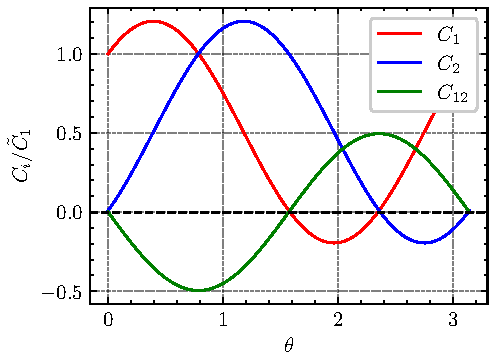
\includegraphics[width=\textwidth]{figures/DC_residue_eig_ratio_0.01.pdf}
    \end{subfigure}
    \caption{Left: Cascade synthesis of the impedance function (\ref{eq:impedance_ex2}). Right: Values of the capacitive elements in the synthesis on the left for $\tilde{C}_1/\tilde{C}_2 = 0.01$ and arbitrary $\theta$.}
    \label{fig:cascade_impedance_ex2}
\end{figure}

While the cascade synthesis does go against the usual convention of trying to obtain a synthesis of purely passive elements, it is extremely useful since it allows us to synthesize lumped element circuits that now consist of only capacitors and inductors. We will see later how this allows us to easily interconnect networks of rational impedance functions. It will also be a crucial part of computing decay rates of resonant modes within our circuit when considering loss through the external ports of our network.

Finally, it is important to note that for all of the impedances that we deal with of the form (\ref{eq:impedance}), we always restrict ourselves to a finite number of resonant modes. If we allow for infinite resonant modes, the capacitance  and inductance matrices in the Lagrangian or Hamiltonian representation of the impedance become infinite in size. Furthermore, these infinite capacitance matrices can result in diverging values for our capacitive elements in the cascade synthesis presented here. For a direct example of this, see Appendix \ref{appendix:cascade_ideal_TL} where we consider the ideal lossless transmission line. However, our restriction to a finite number of poles should not cause any problems as long as we always make sure the truncated impedance function is a good approximation of the true impedance function within the relevant working frequency range of our device. 

\subsection{Analysis of the CL Cascade Network}\label{section:cascade_analysis}
Above we have seen how from the rational impedance function (\ref{eq:impedance}), we can obtain a synthesis in the form of a cascade circuit as shown in Fig.\ \ref{fig:cascade_impedance}. Now we show how to find the answer to the opposite question: How can we obtain the rational impedance function for a circuit of the cascade form shown in Fig.\ \ref{fig:cascade_impedance}? We want to answer this question for any general Maxwell or mutual capacitance matrix along with general values for the inductances shunting the ports of the cascade. Note that here we assume that the Maxwell capacitance matrix we start with is positive definite. Since we know that the impedance function (\ref{eq:impedance}) has a synthesis of the cascade form presented in the last section, we expect that it should be possible to find this function for a general cascade network.

To do this, we start with the Lagrangian for a general cascade with Maxwell capacitance matrix $\vb{C}$ shunted by a set of inductors $L_{R_k}$. With the ports of the cascade network left open, we have the following:
\begin{equation}
    \mathcal{L} = \frac{1}{2}\dot{\vb{\Phi}}^T \vb{C} \dot{\vb{\Phi}} - \frac{1}{2}\vb{\Phi}^T \vb{M} \vb{\Phi}^{\phantom{^T}} \quad\text{where}\quad \vb{M} = \mqty( \vb{0}_{N \times N} & \vb{0}_{N \times M} \\ \vb{0}_{M \times N} & \vb{M}_R ),
\end{equation}
$\vb{M}_R = \diag(1/L_{R_1},\dots,1/L_{R_k})$, and $\vb{\Phi} = (\Phi_{P_1}, \dots, \Phi_{P_N}, \Phi_{R_1}, \dots, \Phi_{R_M})^T$. We will also use the vector $\vb{\Phi}_P$ and $\vb{\Phi}_R$ which contain the port fluxes $\Phi_{P_i}$ and inductor fluxes $\Phi_{R_i}$, respectively. If we look back at the Lagrangian (\ref{eq:impedance_lagrangian}) or Hamiltonian (\ref{eq:impedance_hamiltonian}) corresponding to the synthesis of impedance function (\ref{eq:impedance}), we see there that the diagonal inductance matrix $\vb{M}_R$ contains the frequencies squared of the resonant modes within our network. This is different to the diagonal matrix $\vb{M}_R$ we have here for our general network that just contains the inverse inductances. We want to find a new set of transformed flux variables that also transforms the matrix $\vb{M}_R$ such that its diagonal contains the frequencies squared of the resonant modes rather than the inverse inductances shunting the network. Finding this transformation and applying it to the inductance matrix gives us the resonant modes of the network and thus the poles of the impedance function. Once the poles are found, the same transformation can be applied to the capacitance matrix from which the residues of the impedance function can be extracted using (\ref{eq:impedance_cap}). To find this transformation, we can look at the equations of motion for the flux variables in the Lagrangian:
\begin{equation}
    \vb{C}\ddot{\vb{\Phi}} = -\vb{M} \vb{\Phi} \quad\longrightarrow\quad \ddot{\vb{\Phi}} = -\vb{C}^{-1}\mqty(\vb{0}_N \\ \vb{M}_R \vb{\Phi}_R) = -\mqty( (\vb{C}^{-1})^{\phantom{RP}}_P & (\vb{C}^{-1})^{\phantom{RP}}_{PR} \\ (\vb{C}^{-1})^{\phantom{RP}}_{RP} & (\vb{C}^{-1})^{\phantom{RP}}_R )\mqty(\vb{0}_N \\ \vb{M}_R \vb{\Phi}_R)
\end{equation}
The above gives us the equations of motion for the resonator flux variable block of the inverse capacitance matrix:
\begin{equation}
    \ddot{\vb{\Phi}}_R = -(\vb{C}^{-1})_R \vb{M}_R \vb{\Phi}_R
\end{equation}
To find the transformation described above, we will need to simultaneously diagonalize the matrix product $(\vb{C}^{-1})_R \vb{M}_R$ as the eigenvalues of this product should contain the squared resonant frequencies. Since both the matrices $(\vb{C}^{-1})_R$ and $\vb{M}_R$ are real, symmetric and positive definite, these resonant frequencies will be real and positive. For more on this process, see \cite[Chapter 7.6]{horn_johnson} or \cite[Appendix B.1]{cqed_lecture_notes}.
\newpage
For our case here, we present the whole process of constructing this transformation since the proof easily follows given all the pieces. The steps are as follows:
\begin{enumerate}
    \item Diagonalize $(\vb{C}^{-1})_R = \vb{O}^{\phantom{T}}_C \vb{D} \vb{O}_C^T$.
    \item Define $\vb{T} = \vb{O}_C \vb{D}^{1/2}$.
    \item Diagonalize $\vb{T}^T \vb{M}_R \vb{T} = \vb{O}^{\phantom{T}}_M \vb{\Omega}^2 \vb{O}_M^T$.
    \item Using the above, our needed transformation can be defined as $\vb{S} = \vb{T}\vb{O}_M$.
\end{enumerate}
From the construction above, we can see that $\vb{M}_R = (\vb{S}^{-1})^T \vb{\Omega}^2 \vb{S}^{-1}$ and $\vb{S}\vb{S}^T = (\vb{C}^{-1})_R$. The matrix product then equals $(\vb{C}^{-1})_R \vb{M}_R = \vb{S} \vb{\Omega}^2 \vb{S}^{-1}$. We see that $\vb{S}$ does indeed diagonalize the matrix product. $\vb{S}$ also transforms $\vb{M}_R$ into the diagonal matrix containing the frequencies squared of the resonant modes. With this, we can now define a set of steps to follow that allow us to find the rational impedance function for the general cascade network.
\begin{framed}
\noindent \underline{Finding the Poles and Residues of the Impedance Function for a CL Cascade}
\begin{enumerate}
    \item Find the matrix $\vb{S}$ that diagonalizes $(\vb{C}^{-1})_R \vb{M}_R = \vb{S} \vb{\Omega}^2 \vb{S}^{-1}$.
    \item Define a transformed set of flux variables using $\vb{S}$:
    \begin{equation}
        \vb{\Psi} = \bar{\vb{S}}^{-1} \vb{\Phi} \quad\text{where}\quad \bar{\vb{S}} = \mqty(\mathds{1}_{N \times N} & \vb{0}_{N \times M} \\ \vb{0}_{M \times N} & \vb{S})
    \end{equation}
    This will give the transformed Lagrangian:
    \begin{equation}
        \mathcal{L} = \frac{1}{2}\dot{\vb{\Psi}}^T \bar{\vb{S}}^T \vb{C} \bar{\vb{S}} \dot{\vb{\Psi}} - \frac{1}{2}\vb{\Psi}^T \bar{\vb{S}}^T \vb{M} \bar{\vb{S}} \vb{\Psi}^{\phantom{^T}}
    \end{equation}
    \item Extract the poles of the impedance function from the diagonal matrix 
    \begin{equation}
        \vb{\Omega} = (\vb{S}^T \vb{M}_R \vb{S})^{1/2}
    \end{equation}
    \item Extract the residues of the impedance from the transformed capacitance matrix:
    \begin{equation}
        \bar{\vb{C}} = \bar{\vb{S}}^T \vb{C} \bar{\vb{S}} = \bar{\vb{S}}^T\mqty(\vb{C}_P & \vb{C}_{PR} \\ \vb{C}_{PR}^T & \vb{C}_R )\bar{\vb{S}} = \mqty(\vb{C}_P & \vb{C}_{PR} \vb{S} \\ \vb{S}^T \vb{C}_{PR}^T & \vb{S}^T \vb{C}_R \vb{S})
    \end{equation}
    Since the transformed inductance matrix $\vb{S}^T \vb{M}_R \vb{S}$ will contain the frequencies squared on the diagonal, we can say that the transformed capacitance matrix will be of the form (\ref{eq:impedance_cap}) and we can equate the two:
    \begin{equation}
        \mqty(\vb{C}_P & \vb{C}_{PR} \vb{S} \\ \vb{S}^T \vb{C}_{PR}^T & \vb{S}^T \vb{C}_R \vb{S}) = \mqty( \vb{R}_0^{-1} & -\vb{R}_0^{-1}\vb{R}^T \\ -\vb{R} \vb{R}_0^{-1} & \mathds{1}_{M\times M} + \vb{R}\vb{R}_0^{-1}\vb{R}^T)
    \end{equation}
    Equating the two matrices tells us that the DC residue of the impedance function for this network is $\vb{R}_0 = \vb{C}_P^{-1}$. Then, using equality of the port-resonator block of the matrices above, we can compute the turns ratio matrix $\vb{R}$:
    \begin{equation}
        \vb{R} = -(\vb{C}_P^{-1} \vb{C}_{PR} \vb{S})^T = -\vb{S}^T \vb{C}_{PR}^T \vb{C}_P^{-1}
    \end{equation}
    As explained earlier, the rows $\vb{r}_k$ of this turns ratio matrix can be used to obtain the residues $\vb{R}_k = \vb{r}_k^T \vb{r}_k$ of the impedance function.
\end{enumerate}
\end{framed}
\newpage
With all of the steps above, we can construct the rational impedance function for a general CL cascade network. To show that this does in fact work, we can compare the method of finding the rational impedance function to a method for computing the S-parameter of a cascade-loaded network. Here we briefly go over this method as we will see it will also be useful later on when adding elements at the ports of our networks.

\begin{figure}[h!]
    \centering
    \begin{circuitikz}[line width=1pt]
        \ctikzset{bipoles/thickness=1, bipoles/length=1cm}
        \ctikzset { label/align = straight }
        
        % ---------------------------- Capacitive Network ---------------------------- %
        \draw[rounded corners=.5cm] (0,2) -- (0,4.5) -- (6,4.5) -- (6,0) -- (0,0) -- (0,2);
        \node at (2.5,2.25) {\large $\vb{\Sigma} = \mqty(\vb{\Sigma}_{11} & \vb{\Sigma}_{12} \\ \vb{\Sigma}_{21} & \vb{\Sigma}_{22})$};

        % --------------------------- Inductive Network Box -------------------------- %
        \draw[rounded corners=0.5cm] (8,2) -- (8,4.5) -- (10,4.5) -- (10,0) -- (8,0) -- (8,2);
        \node at (9,2.25) {\large $\vb{S}_\ell$};

        % ------------------------------ Left Lower Port ----------------------------- %
        \draw (0,0.5) to[short, -o] (-1,0.5);
        \draw (0,1.5) to[short, -o] (-1,1.5);

        % ------------------------------ Left Upper Port ----------------------------- %
        \draw (0,3) to[short, -o] (-1,3);
        \draw (0,4) to[short, -o] (-1,4);

        % ----------------------------- Middle Lower Port ---------------------------- %
        \draw (6,0.5) to[short, -o] (7,0.5) -- (8,0.5);
        \draw (6,1.5) to[short, -o] (7,1.5) -- (8,1.5);

        % ----------------------------- Middle Upper Port ---------------------------- %
        \draw (6,3) to[short, -o] (7,3) -- (8,3);
        \draw (6,4) to[short, -o] (7,4) -- (8,4);

        \node at (-0.5,2.35) {$\vdots$};
        \node at (7,2.35) {$\vdots$};

        \draw[decoration={brace}, decorate] (-1.25,0.25) -- (-1.25,4.25);
        \node[rotate=90] at (-1.75, 2.25) {$N$ ports};

        \draw[decoration={brace}, decorate] (5.5,0.25) -- (5.5,4.25);
        \node[rotate=90] at (5, 2.25) {$M$ ports};


    \end{circuitikz}
    \caption{General cascade loaded network.}
    \label{fig:general_cascade_load}
\end{figure}

Consider the general cascade-loaded network as shown in Fig.\ \ref{fig:general_cascade_load}. The left $(N+M)$-port network in the cascade has the S-parameter $\vb{\Sigma}$ and the load has an $M$-port S-parameter $\vb{S}_\ell$. $\vb{\Sigma}$ can be broken up into blocks that correspond to external and internal ports. The S-parameter $\vb{S}$ of the loaded network can then be computed using \cite[Eq. 3.20]{newcomb}:
\begin{align}\label{eq:cascade_s}
    \vb{S} = \vb{\Sigma}_{11} + \vb{\Sigma}_{12}\vb{S}_\ell (\mathds{1}_{M \times M} - \vb{S}_{22}\vb{\Sigma}_\ell)^{-1}\vb{\Sigma}_{21}= \vb{\Sigma}_{11} + \vb{\Sigma}_{12} (\mathds{1}_{M \times M} - \vb{S}_\ell\vb{\Sigma}_{22})^{-1}\vb{S}_\ell\vb{\Sigma}_{21}
\end{align}

To use the above formula to find the S-parameter of the CL cascade, we can use the impedance functions for the purely capacitive network and the inductive shunt network. The impedance function of the $(N+M)$-port capacitive network is $\vb{Z}_C(s) = \vb{C}^{-1}/s$. For the $M$-port inductive shunt network, the impedance function is $\vb{Z}_L(s) = s\vb{L}$ where $\vb{L} = \diag(L_1,\dots,L_M)$. Converting each of these impedance functions to S-parameters allows us to use (\ref{eq:cascade_s}) to compute the S-parameter of the cascaded network discretized in frequency. The final S-parameter can be converted back to an impedance function and then compared to our expected rational impedance function.  

In Fig.\ \ref{fig:rand_impedance_ex}, we take a randomly generated CL cascade network and compute the poles and residues of the rational impedance function using the method discussed above. Then we compare it to the impedance function computed using (\ref{eq:cascade_s}) and the S-parameters of the capacitive and inductive networks. We see that the difference between the two is quite small in the chosen frequency range with some larger deviations around the poles. This is due to numerical error that arises in computing the pole locations and the conversions between S and Z-parameters.

\begin{figure}[h!]
    \centering
    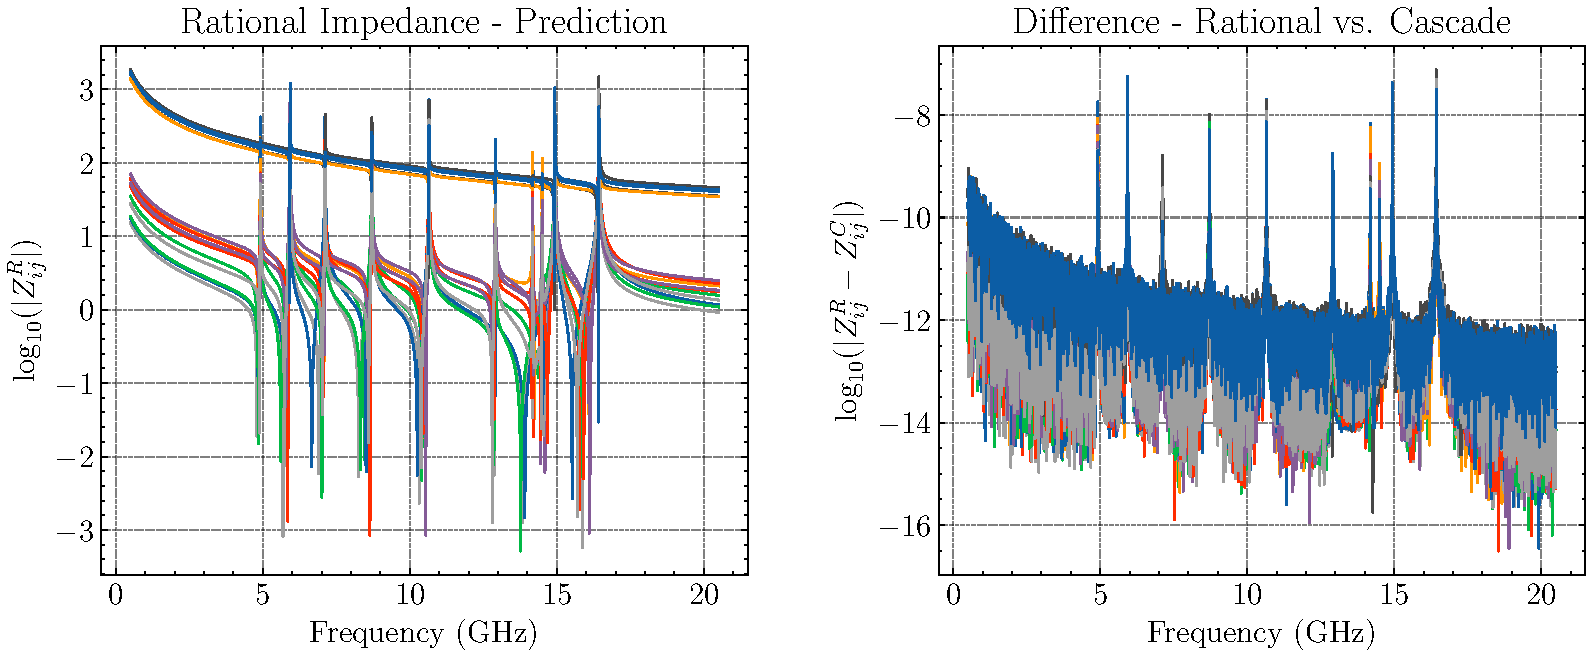
\includegraphics[width=\textwidth]{figures/5_port_10_res_rand.pdf}
    \caption{Left: Rational impedance function $\vb{Z}^R$ with 5 ports and 10 resonant modes. The capacitive network and inductive shunts are randomly generated. Port shunt capacitors are between 100 and 200 fF, and port coupling capacitances are between 0 and 10 fF. Shunt inductors are between 0.4 and 5 nH. Right: The difference between the predicted rational impedance function $\vb{Z}^R$ and the discretized cascade impedance $\vb{Z}^C$ computed using (\ref{eq:cascade_s}).}
    \label{fig:rand_impedance_ex}
\end{figure}

If we know the capacitance matrix and shunt inductor values, then we can already write a Hamiltonian for the CL cascade network so we do not necessarily need to find the rational impedance function. However, it is useful to have a clear method for calculating the resonant frequencies of the network. Furthermore, we will see in the next section that this method can be used to recover the rational impedance function of an interconnected network of rational impedances.